\documentclass[]{aiaa-tc} % insert '[draft]' option to show overfull boxes

 \title{Gradient-Based Optimization on Large Design Spaces with Graph-Based Problem Formulation In OpenMDAO}

\author{
  Tristan A. Hearn,%
     \thanks{Aerospace Engineer, MDAO Branch, Mail Stop 5-10, AIAA Member}
  \ Kenneth T. Moore,%
     \thanks{Senior Systems Engineer, MDAO Branch, Mail Stop 500-105, AIAA Senior Member}
  \ Justin Gray,%
     \thanks{Aerospace Engineer, MDAO Branch, Mail Stop 5-11, AIAA Member}
   \\
  {\normalsize\itshape
  NASA Glenn Research Center, Cleveland, OH}  \\
 }

\AIAAconference{Multidisciplinary Design Optimization Specialist Conference}
\AIAAcopyright{\AIAAcopyrightD{2012}}


% Define commands to assure consistent treatment throughout document
\newcommand{\eqnref}[1]{(\ref{#1})}
\newcommand{\class}[1]{\texttt{#1}}
\newcommand{\package}[1]{\texttt{#1}}
\newcommand{\file}[1]{\texttt{#1}}
\newcommand{\BibTeX}{\textsc{Bib}\TeX}

\setlength{\abovecaptionskip}{0pt}
\setlength{\belowcaptionskip}{0pt}

\usepackage{setspace}

\usepackage{graphicx}
\usepackage{wrapfig}
\usepackage{caption}
\usepackage{amsmath}
\usepackage{lscape}
\usepackage{hyperref}
\usepackage{minted}
\usepackage{color}
\usepackage{appendix}
\usepackage[section]{placeins}


\captionsetup[figure]{margin=5pt,font=small,labelfont=bf,textfont=bf,justification=justified,}
%\captionsetup[wrapfigure]{margin=5pt,font=small,labelfont=bf,justification=justified,singlelinecheck=off}
\captionsetup[table]{margin=5pt,font=small,labelfont=bf,textfont=bf,justification=justified,position=top}

\bibliographystyle{aiaa}

\usepackage{lettrine}
\usepackage{verbatim}

\begin{document}

  \maketitle

  \begin{abstract}

  \end{abstract}

  \section{Introduction}

    Many of today's the most interesting design problems involve very large design spaces with 100's or 1000's of
    design variables. Large design spaces are often approached through the use of gradient based optimization
    analytic derivatives to achieve highly scalable solution strategies. For instance, adjoint based gradient
    methods have allowed CFD based shape optimization to tackle problems with 100's of design variables. [Cite Juan's Groups
    work here]. Coupled Aero-structural optimization is another area where gradient based optimization methods have
    been employed. [Cite Martins groups work here]. Although these problems have large design spaces,
    they include only a few disciplines (i.e. Geometry, Aerodynamics, Structures). The relative simplicity of
    the problem formulation make it feasible to use custom implementations tailored to a specific problem. These specific
    implementations make it difficult to modify the problem formulation without significant effort. For problems
    with more disciplines customs solutions become less feasible, and a more general means of setting up
    the design problem is required.

    In this work we demonstrate how OpenMDAO, an open-source MDAO framework, provides a more general
    solution to constructing and solving complex problems with large design spaces. Use of OpenMDAO
    provides benefits in a number of important respects:

    \begin{enumerate}
      \item Combining analytic derivatives with finite difference in a mixed derivatives environment
      \item Automatic and efficient solving for the coupled derivatives at the system level
      \item Automatic assembly of the full gradient from the partial derivatives of each discipline
      \item Flexbility via separation of problem formulation from solution strategy
      \item Simple implementation for multi-point design problems
    \end{enumerate}

    The approach used in OpenMDAO is maintain a central, monolithic, data connectivity graph between all
    variables and components in the model. The graph utilizes the structure proposed by Pate et. al \cite{graph_problem2013}
    and represents the complete problem formulation as defined by the user. The graph is then used in order to
    facilitate all of the five features described above. The

  \section{Problem Formulation Graph}

    One key technology that enables the flexible solution of an MDAO problem is the representation
    of its dataflow as a dependency graph. A dependency graph is a directed network graph whose
    edges represent the dependencies between its nodes. In a framework, an input needed by one
    discipline must be provided by the output of another. This is a dependency, and is represented
    in a dependency graph containing nodes for the output and input, and an directional edge
    between them. It is clear that the upstream discipline must provide the output before the
    downstream one can receive it, and this directional information is contained in the dependency
    graph.

    The main advantage of tight integration with a dependency graph is the availability of efficient
    algorithms for performing a number of functions that are useful for solving an MDAO problem.

      1. Determination of component execution order.
      2. Identification of cycles.
      3. Identification of parallel structures.
      4. Determination of driver subgraphs.

    The OpenMDAO framework uses a dependency graph to determine component execution order and to
    drive the process of invalidation, which finds the minimum set of components that needs to
    be re-executed when a set of inputs change. (ref: last OpenMDAO paper.) A dependency graph
    can also identify cycles in the graph, and hence a cycle in the dataflow that must be resolved
    by a solver. Similarly, the graph can also be used to examine the potential for parallelism at
    a component level.

    The determination of driver subgraphs is a capability that will be investigated in this paper.
    Consider an optimizer with n parameters, 1 objective, and m constraints. The relevant
    subgraph of this problem is the set of component disciplines and their variable connection that
    lie within the subgraph between the parameters and the constraints and objective. This subgraph
    contains the components that execute when the optimizer requests a function evaluation. It is
    also useful for setting up and solving the coupled derivative system when the optimizer requests
    a gradient evaluation. For calculation of the coupled derivative in adjoint mode, further
    efficiency can be gained by using the subgraph that includes just the portion of the graph
    between a single constraint and the parameters. Similarly for forward mode, the subgraph would
    include just the portion of the graph between a single parameter and the constraints/objective.

    [Intro to OpenMDAO paragraph]

    [Derivatives in OpenMDAO paragraph]


    \subsection{Fake Finite Difference}
    \subsection{Relevant Variable Identification}

  \section{CADRE Problem Formulation}

  \section{CADRE Results}

The OpenMDAO implementation of the CADRE problem was executed on a Macbook Pro[specs]
over the course of two days, to a termination tolerance of $10^{-5}$. This tolerance
was achieved within approximately 106 iterations, using the SNOPT\cite{gill2005snopt}
optimizer.

\begin{figure}
\centering
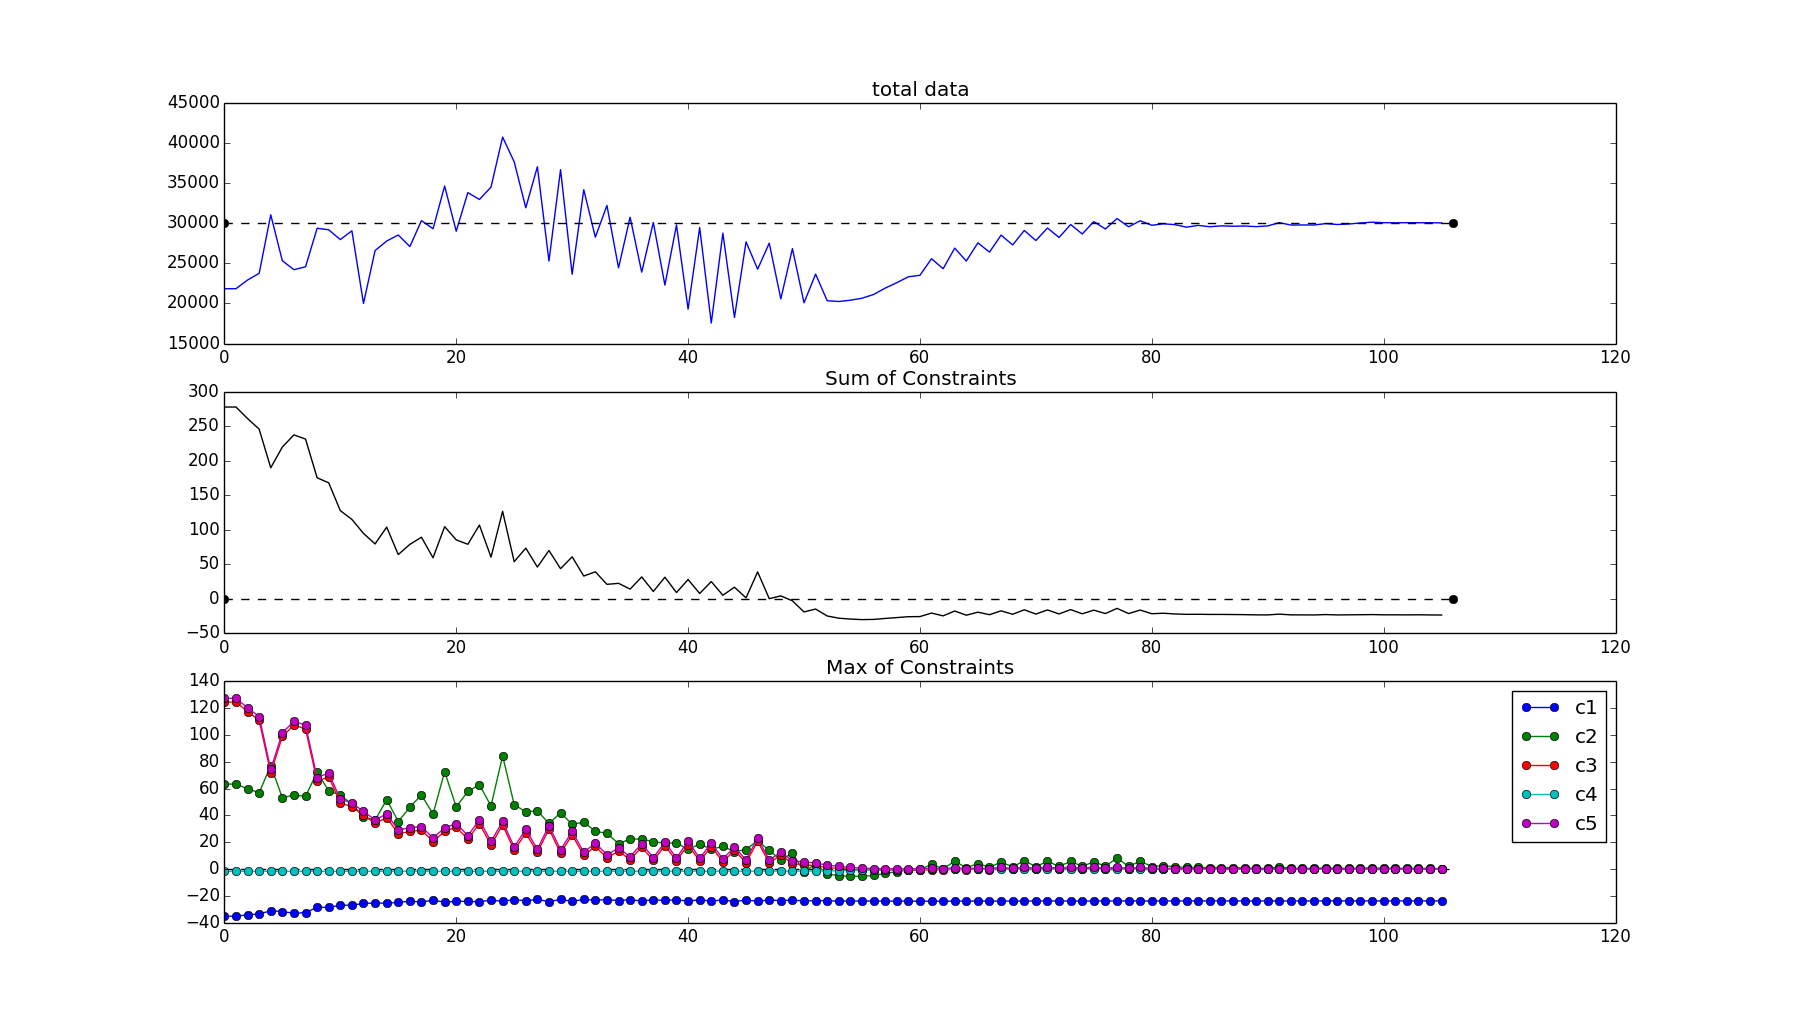
\includegraphics[width=0.99\textwidth]{images/opt.png}
\caption[width=0.22\textwidth]{Convergence of the CADRE problem.}
\label{convergence}
\end{figure}


Figure \ref{convergence} illustrates the convergence of the CADRE problem over the course of
these iterations. The first row plots the
value of the objective function, the total data downloaded over each design point. The objective
function oscillated greatly over the course of the first half of the computed iterations, but
stabilized by the 80th iteration near the value previously determined[cite CADRE paper]
to be the optimal design.

The second row plots the maximum value of each constraint across all design points at
each iteration. As all of the problem constraint are non-positive for a feasible design,
this can be taken as a cursory measure of overall problem feasibility.
The third row plots the maximum value of each constraint across each of the design points,
but separated according to specific constraint type. These two plots both indicate that the
oscillatory behavior of the objective function coincided with a steady decrease in design
infeasibility. Once a feasible state was reached (near the 50th iteration), the optimizer
began refining the design towards a more favorable value of the objective function.

\begin{figure}
\centering
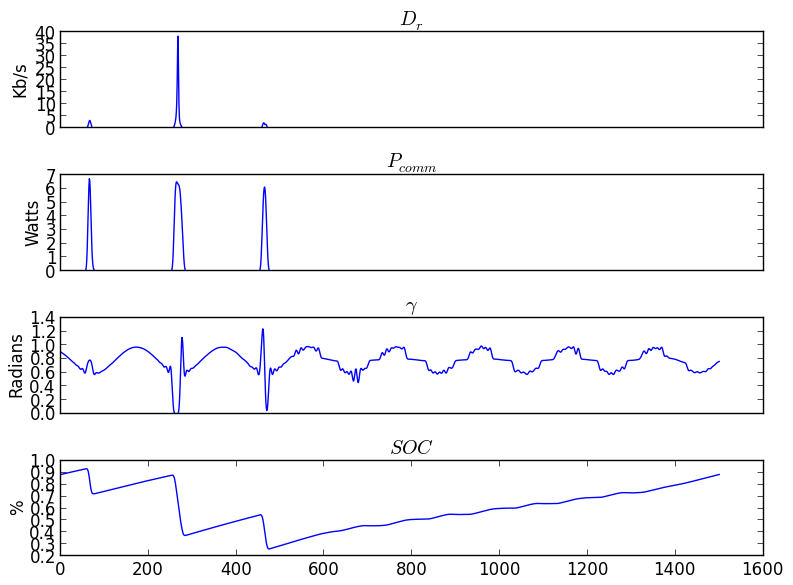
\includegraphics[width=0.8\textwidth]{images/pt_3_data.png}
\caption[width=0.4\textwidth]{Plots of the bit rate, communications systems power, craft roll angle,
and battery charge level over the half-day time period covered by the $4^{\textrm{th}}$ design point.}
\label{pt3_data_results}
\end{figure}

Figure \ref{pt3_data_results} shows plots of selected variables for the $4^{\textrm{th}}$ design points,
to illustrate the fidelity of the recovered solution. These variables are the communications bit rate ($D_r$), communications systems power level ($P_{comm}$), craft roll angle ($\gamma$),
and battery charge level ($SOC$). These variables were each instantiated to uniform values
(across all time points) of 0, 0, $\frac{\pi}{4}$, and 0 respectively. The optimizer, operating on
OpenMDAO's graph formulation of the problem succeeded at converging each of these variables to the values
shown, for each time point.

Further post processing of the data included automatic geographical rendering of the trajectories of
the CADRE satellite for each of the 6 design points, using the Google
Maps\footnote{http://developers.google.com/maps/} and Google
Earth\footnote{http://developers.google.com/earth/} APIs. The trajectories are
represented as polygonal chain ("polyline") elements, colored according to the
satellites communication bitrate with the ground station during the corresponding
window of time.

Each time point is represented by two separate polyline objects with endpoints
at the location of the satellite at that moment in time. One polyline element terminates
halfway between this location and the location at the preceding moment in time,
and the other between this and the location at the next moment in time. This way,
the colored line segments seen on the figures are appropriately centered on the
locations determined by the time points when the data bit rate values were calculated
by the OpenMDAO model.


\begin{figure}
\centering
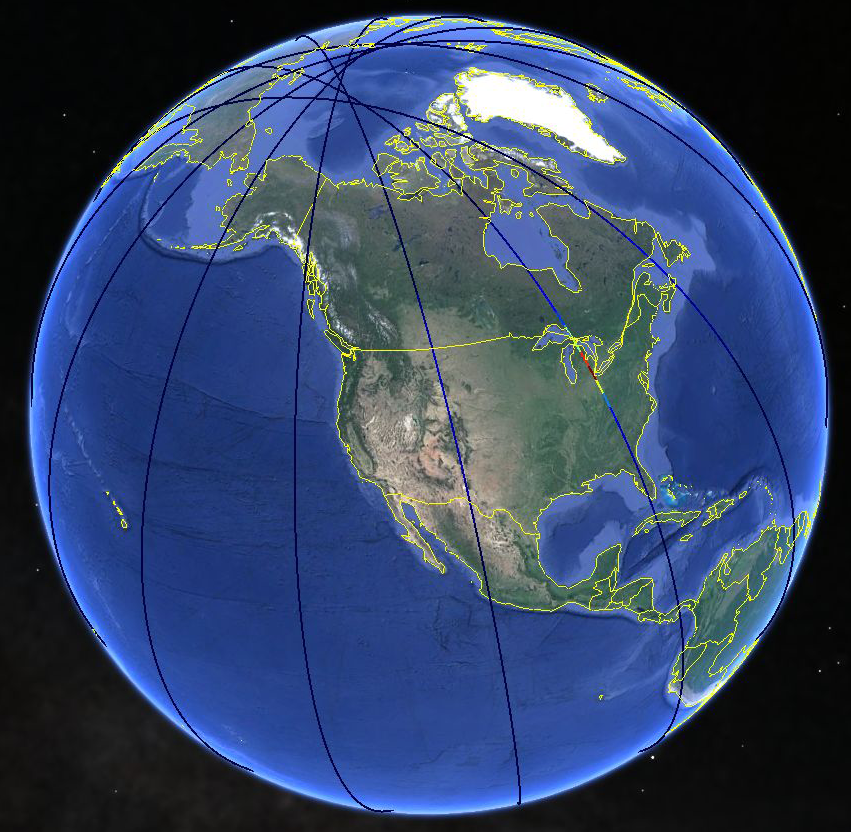
\includegraphics[width=0.9\textwidth]{images/pt3_gearth3.png}
\caption[width=0.4\textwidth]{Plot of the trajectories of the CADRE satellite
for the $4^{\textrm{th}}$ design point onto the surface of the Earth, illustrating the
communication data rates near the ground station.}
\label{pt3_g_earth}
\end{figure}


\begin{figure}
\centering
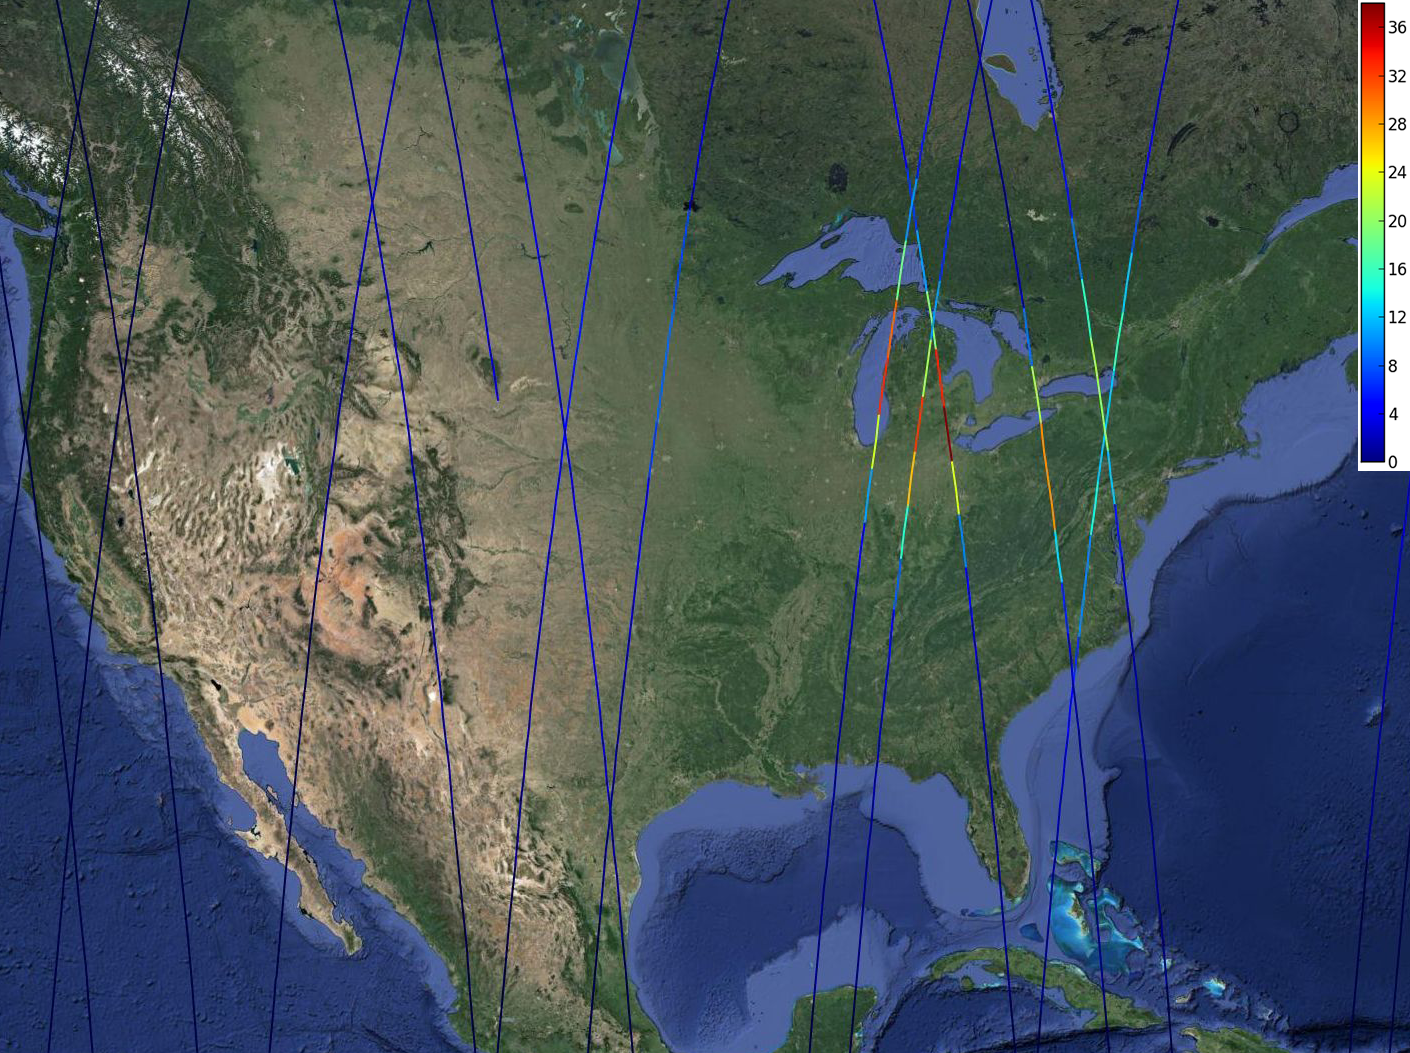
\includegraphics[width=0.9\textwidth]{images/allpts_map_data.png}
\caption[width=0.4\textwidth]{Plot of the trajectories of the CADRE satellite
for all 6 design points onto the surface of the Earth, illustrating the
communication data rates near the ground station.}
\label{pt3_g_earth}
\end{figure}


\begin{figure}
\centering
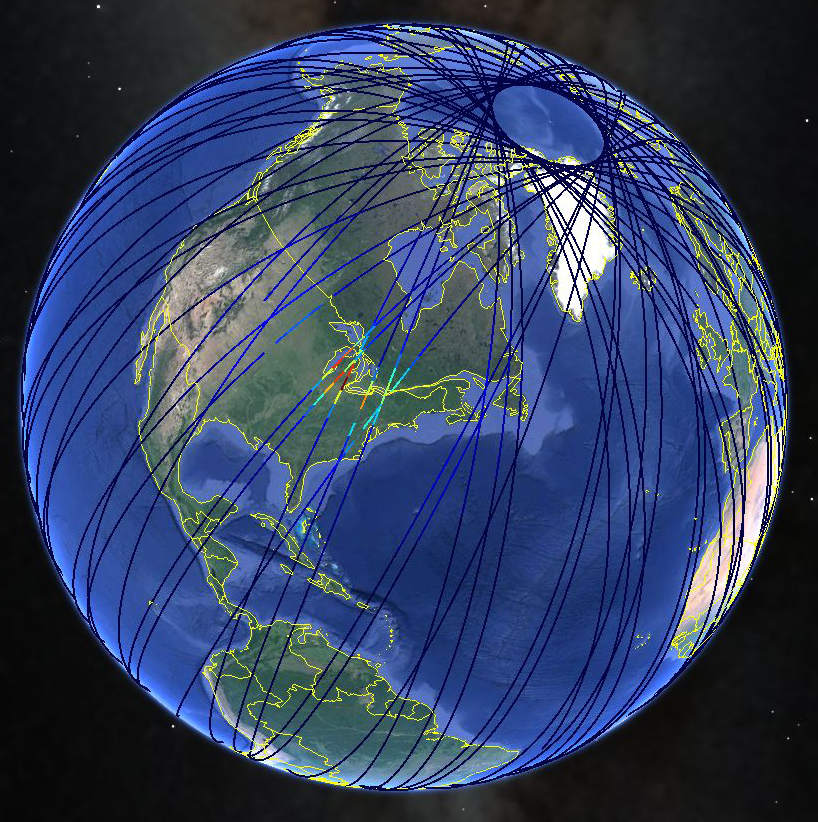
\includegraphics[width=0.9\textwidth]{images/allpts_gearth2.png}
\caption[width=0.4\textwidth]{Plot of the trajectories of the CADRE satellite
for all 6 design points onto the surface of the Earth.}
\label{pt3_g_earth}
\end{figure}


  \section{Aero-Structural Problem Formulation}

  \section{Aero-Structural Results}

  \section{Conclusion}

  \bibliography{references}


\end{document}
